\section{Ejercicio 8}

Se decidió separar el diseño en varios bloques que cumplieran tareas específicas, facilitando la implementación. Para comenzar, para evitar problemas de ruido se dividió la implementación en parte digital y analógica.\par
Los bloques utilizados fueron un generador de rampa con un comparador, un contador para la tasa de refresco y otro contador como elemento de medición. Su propuesta de diseño e implementación se presentan a continuación. \par
Se realizaron simulaciones en LTSpice, Proteus y Verilog de las distintas secciones del circuito para validar y confeccionar el circuito planteado a continuación.

\subsection{Diseño}

\subsubsection{Consideraciones generales}

Para comenzar, se decidió implementar todo el circuito en un único PCB para mayor eficiencia y claridad. Se consideró que la previa modularización del circuito en las partes mencionadas anteriormente, un trabajo de ruteo a conciencia y eficiente y medidas para atenuar el ruido, harían posible implementar todo el circuito en la misma placa. \par De esta manera, con la finalidad de reducir la injerencia del ruido, se dividió la placa en dos secciones, una para la parte digital y otra para la analógica. La sección analógica está compuesta por el generador de rampa, comparadores(opamps) y un generador de clock. Por otro lado, la sección digital está compuesta por contadores, comparadores, decodificadores y diversas compuertas lógicas discretas. También, se realizaron dos planos de masa independientes, uno para cada sección. Como tercera medida, la alimentación de ambas secciones se realizó en la misma bornera pero sin juntar las pistas, estando conectadas directamente a la misma sin contacto previo. \par 


Por otro lado, se utilizaron dos tensiones de alimentación de $5\,V$ y $15\,V$. La primera para alimentar los circuitos integrados lógicos como las compuertas AND, XOR, entre otras. Mientras que fue necesario una tensión mayor para alimentar el circuito integrado $NE\,555$, el generador de la rampa, y diversos amplificadores operacionales.\par

Respecto al diseño del circuito per se, se implementó una rampa de frecuencia constante que funcionará como referencia para el proceso de conteo, pudiendo entrar la cantidad necesaria de mediciones para cubrir el espectro solicitado por la cátedra para cada rampa. Luego, se utilizó un sistema con un contador, un comparador, entradas externas digitales y compuertas lógicas discretas para variar la tasa de refresco, habilitando o deshabilitando las mediciones asociadas a la rampa. \par 

Fue indispensable utilizar amplificadores operacionales diseñados especialmente para funcionar como comparadores($LM339$) ya que las condiciones donde tienen que reaccionar son de duración extremadamente corta como el caso del reset que se verá más adelante. Para ello es necesario un tiempo de respuesta extremadamente breve capaz de llegar a detectar y variar en esa estrecha ventana de tiempo.


\subsubsection{Generador de Rampa}

Primeramente, se necesitó medir de cierta manera la variación en la tensión provista por el joystick, la cual será proporcional a su posición respecto del eje. Esto se debe a que internamente el joystick cuenta con un pontenciómetro que provee entre $0\,V$ y $5\,V$ de voltaje de salida. Por ende, se diseñó una rampa utilizando un circuito integrado $NE\,555$, la misma se utilizará para comparar tensiones. \par

\begin{figure}[H]
\centering
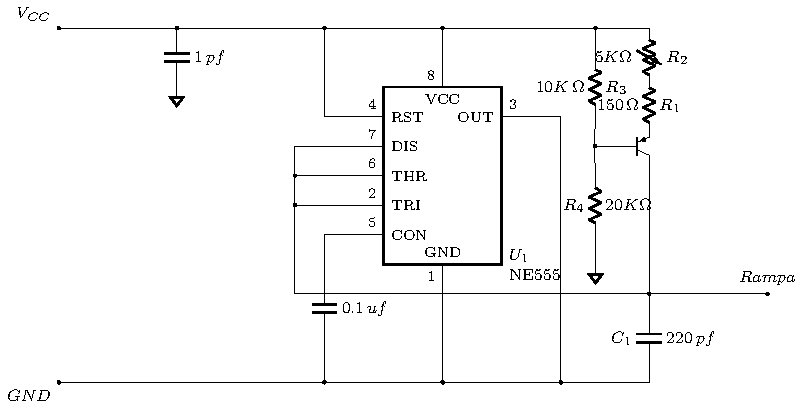
\includegraphics[scale=0.8]{Ejercicio8/Circuitos/Generador_de_rampa.pdf}
\caption{Generador de Rampa con desfasaje}
\label{fig:Generador_de_rampa}
\end{figure}

La rampa representará la carga del capacitor $C_1$ presente en el circuito (\ref{fig:Generador_de_rampa}), dicha carga será constante debido a que el componente anteriormente mencionado está conectado con el colector del transistor PNP que está actuando como fuente de corriente. La tasa de refresco estará dada por la frecuencia de la rampa, siendo la misma constante y de $20\, Hz$. \par
La pendiente $S$ de la rampa estará dada por $S=\frac{I_C}{C_1}=\frac{\Delta V}{\Delta t}$.
Para comenzar, se decidió fijar el valor de $C_1$ en $22\,uf$ tal que sólo sea variable $I_C$. Por otro lado, la corriente en el colector está dada por:

\begin{equation}
I_C=\frac{V_{CC}-V_E}{R_E}
\end{equation}

La tensión en el emisor está determinada por un divisor resistivo dado por:

\begin{equation}
V_E=\frac{R_4}{R_4+R_3} V_{CC} + V_{BE}
\end{equation}
\par
Se fijaron los valores de $R_4$ y $R_3$ en $20K\,\Omega$ y $10K\,\Omega$ respectivamente, tal que la única incógnita sea $R_E$. \par
Se obtuvo un valor nominal para $R_E$ de $2K\,\Omega$. 
Como primer problema a solucionar para el diseño, surgió que rampa provista por el $NE\,555$ se encontraba entre $5\,V$ y $10\,V$ como se puede ver en la imagen (\ref{fig:Generador_de_rampa_desfasada_LTSpice}). Esto se debe a la construcción propia del integrado que utiliza comparadores para obtener una señal de salida entre un tercio y dos tercios de la tensión de alimentación ($V_{CC}$), en nuestro caso, $15\,V$.


\begin{figure}[H]
\centering
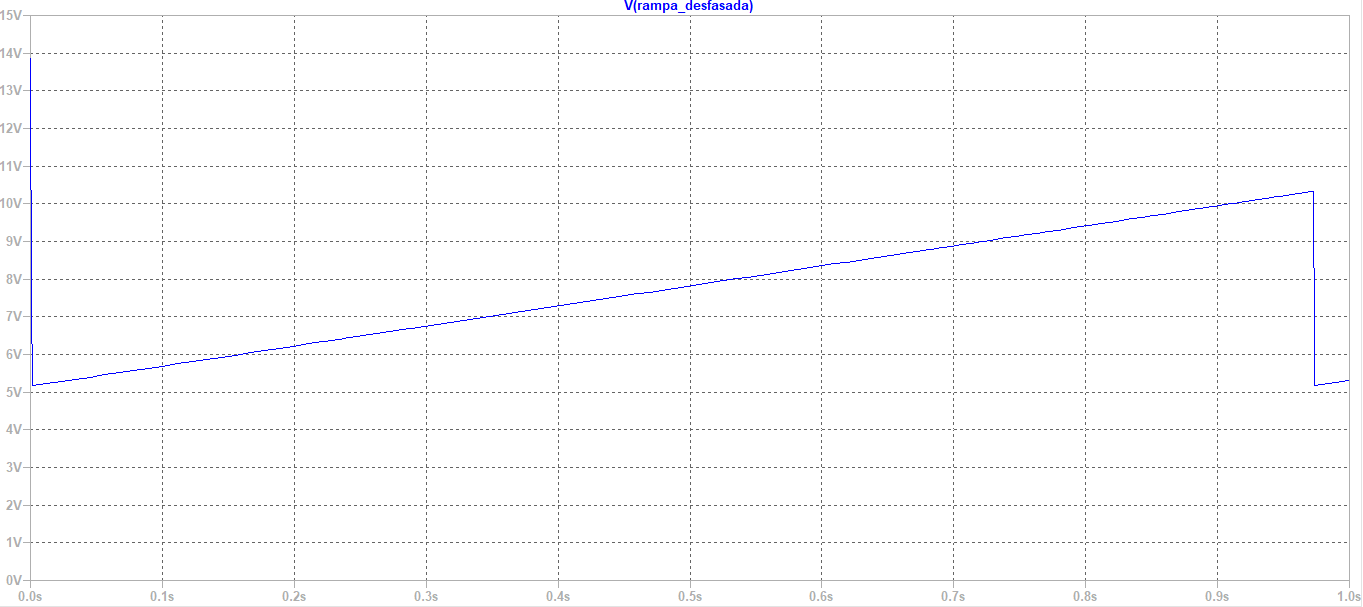
\includegraphics[width=0.7\textwidth]{Ejercicio8/Imagenes/Rampa_desfasada}
\caption{Tensión de la rampa con desfasaje}
\label{fig:Generador_de_rampa_desfasada_LTSpice}
\end{figure}

Por ende, se implementó un amplificador operacional que funcionará como restador para reducir la tensión de salida de la rampa en $5\,V$, utilizando el siguiente circuito:

\begin{figure}[H]
\centering
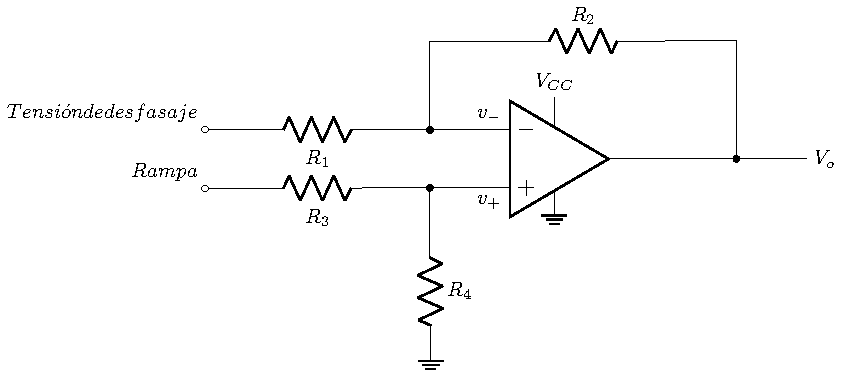
\includegraphics[scale=0.8]{Ejercicio8/Circuitos/Restador.pdf}
\caption{Restador}
\label{fig:Restador}
\end{figure}
\par
La salida del amplificador operacional va a estar dada por:
\begin{equation}
V_o=\frac{-R_2}{R_1}\,V_2+\left(1+\frac{R_4}{R_3}\right)\,V_1
\end{equation}
Tomando valores de resistencias equivalentes de $1\,K\Omega$, obtendremos:
\begin{equation}
V_o=2V_1-V_2
\end{equation}
Siendo $V_1$ la tensión de la rampa y $V_2$ la tensión de desfasaje.\par\par\par
Se obtuvo la siguiente rampa acorde a las necesidades para el trabajo:

\begin{figure}[H]
\centering
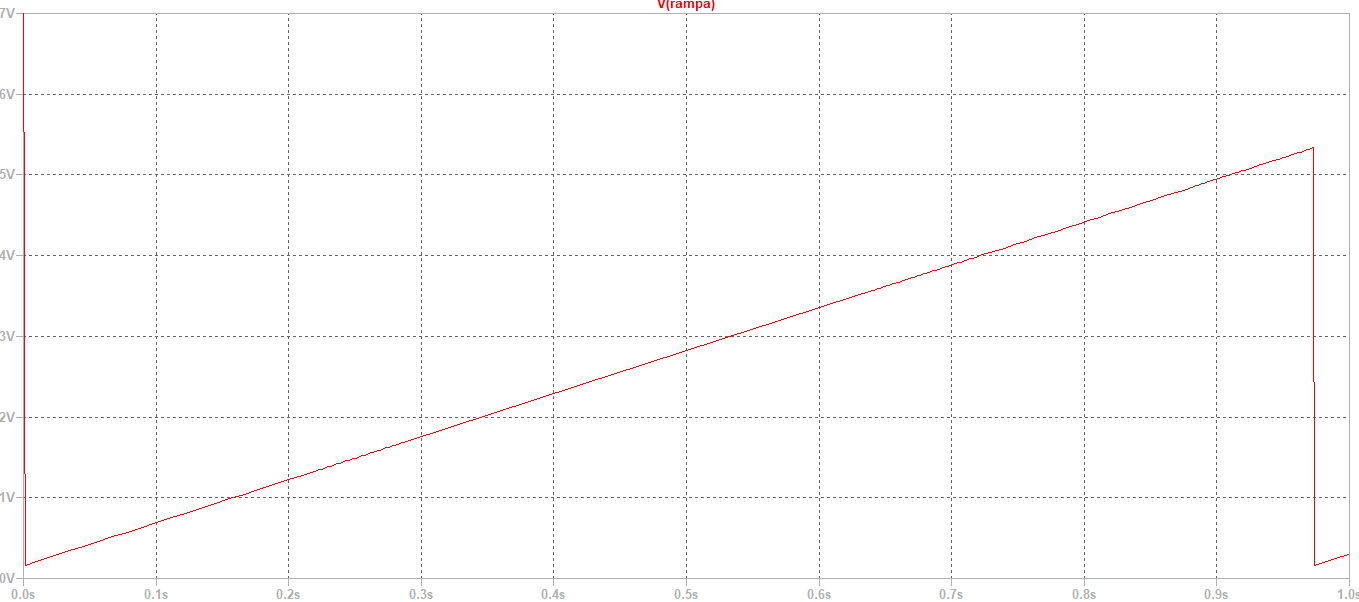
\includegraphics[width=0.7\textwidth]{Ejercicio8/Imagenes/Rampa}
\caption{Tensión de la rampa}
\label{fig:Generador_de_rampa_LTSpice}
\end{figure}



Se considera necesario aclarar la utilización de un buffer entre la salida de la rampa desfasada y el restador para que no se modifiquen los comportamientos entre ambos circuitos. Por otro lado, la pendiente simulada no coincidía con la obtenida empíricamente, siendo esta última irregular con deformaciones debido probablemente a componentes capacitivos parásitos. En vista de este problema, se procedió a reemplazar las resistencias del restador por resistencias variables (presets multivueltas) para calibrar y obtener la rampa idónea para la tarea, es decir, que cuya pendiente sea lo más regular posible.


Como segunda decisión de diseño, se implementó un comparador entre la tensión del joystick y la tensión de la rampa. La tensión del joystick variará respecto del tiempo, motivo por el cual se agrega un filtro pasabajo como se puede observar en la figura (\ref{fig:Comparador}) para estabilizar la señal y disminuir el ruido. Al contar el joystick con un potenciómetro, sólo es necesario agregar un capacitor  a la entrada no inversora del amplificador operacional y tierra, se eligió un capacictor de $1\,uf$.\par
La señal de la rampa estará conectada a la entrada inversora del opamp, mientras que la tensión del joystick estará conectada a la entrada no inversora. \par 
Fue necesario agregar un capacitor y una resistencia de pull up como se indica en la hoja de datos del componente, se puso una resistencia variable de $100\,K\Omega$ para poder calibrar la respuesta ideal del comparador.

\begin{figure}[H]
\centering
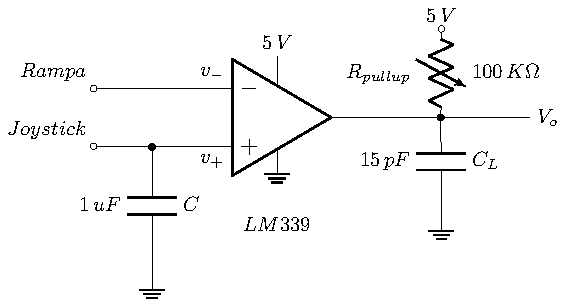
\includegraphics[scale=0.8]{Ejercicio8/Circuitos/Comparador.pdf}
\caption{Comparador de tensiones}
\label{fig:Comparador}
\end{figure}

De esta manera, cuando la tensión de la rampa sea menor a la tensión del joystick la salida del comparador será de $5\,V$, que representará el 1 lógico del circuito digital. Para el caso contrario, la tensión de salida será de $0\,V$, un 0 lógico para el circuito.

\subsubsection{Tasa de refresco}

Fue solicitado por la cátedra una tasa de refresco variable entre $1\,Hz$ y $20\,Hz$. Considerando la limitación de que la frecuencia de la rampa utilizada es fija, va a ser necesario controlar en que momentos se mide, para implementar dicha características se consideraron dos posibilidades. \par

La primera fue una entrada digital, esto se logra mediante un switch de 5 vías conectado a la alimentación($5\,V$) . De esta manera, el usuario puede ingresar de manera manual el número en binario de la tasa de refresco abriendo o cerrando vías del switch hasta encontrar la tasa deseada.
\par

La segunda posibilidad analizada fue implementar un divisor resistivo como se puede observar en la figura (\ref{fig:Divisor}). Se mediría la tensión que cae en $R_1$, que sería entre $0\,V$ y $5\,V$, para luego, mediante un diseño similar al utilizado para el joystick, contar entre 1 y 20 según la tensión medida.

\begin{figure}[H]
\centering
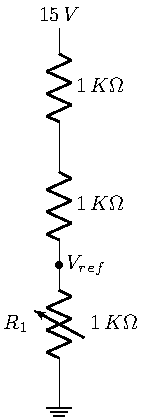
\includegraphics[scale=0.6]{Ejercicio8/Circuitos/Divisor.pdf}
\caption{Reset}
\label{fig:Divisor}
\end{figure}

Finalmente, se decidió implementar sólo la entrada digital, siendo su par analógico descartado por falta de tiempo, aunque se dejaron las conexiones pertinentes por si se realizara en un futuro.\par 

Fue necesario comparar la frecuencia provista por el usuario con la frecuencia de referencia de nuestro circuito representada por la rampa. Por ende, se procedió a derivar la rampa con una compuerta NOT de tecnología Schmitt trigger obteniendosé una señal cuadrada de igual frecuencia. Consiguientemente, mediante un contador se midió la cantidad de pulsos de dicha señal cuadrada a lo largo del tiempo, la señal de clock para dicho contador es la rampa derivada mencionada anteriormente, por lo que nuestro sistema de tasa de refresco se encuentra en sincronía con la rampa y su sistema de medición. Fue necesario utilizar dos contadores BCD (provistos por el integrado $CD4518$) ya que era necesario poder contar hasta 20.  \par 

Como siguiente paso, fue necesario comparar el valor de dicho contador con nuestra entrada digital provista por el usuario mediante un circuito digital comparador $74LS85$ y una compuerta XNOR ($CD4070$). La implementación de la compuerta XNOR fue necesaria debido a que el único comparador digital disponible era uno de 4 bits, cantidad insuficiente para cubrir todo el espectro posible de tasa de refresco, considerando que del 16 al 20 se requieren 5 bits para su representación binaria. \par 

Al detectar que ambos eran iguales, mediante una compuerta AND cuyas entradas son la XNOR y la salida del comparador que indica que ambos números ingresados son iguales, ese era el momento indicado para empezar a contar con la tasa de refresco deseada. Considerando que era necesario resetear el circuito inmediatamente después de dicho pulso y al ser el reset de los contadores asincrónico, fue imperante colocar un Flip Flop D para resolver dicho inconveniente, logrando obtener un delay de un pulso que nos permitiera contar, para luego reiniciar el circuito planteado. \par

Recordando que la frecuencia de la rampa es fija y cada cuanto habilitamos el enable del contador asociado a la misma determina las mediciones de la posición del joystick y  nuestra frecuencia de muestreo, es necesario mencionar que el usuario realmente no está ingresando la misma sino que ingresa la cantidad de pulsos que se debe esperar para contar. A modo de ejemplo, para una espera de 1 pulso, se contará durante un pulso si y durante otro no, dando una frecuencia de muestreo de $10\,Hz$ o para una espera de 4 pulsos la tasa será de $4\,Hz$, y así sucesivamente. \par
 
Es indispensable considerar el comportamiento del circuito al momento que el usuario decida introducir un nuevo valor mediante los switches,  cambiando la cantidad de los pulsos de espera. Si el usuario ingresará un número mayor al original no existiría inconveniente ya que sólo cambiará el número hasta el que el contador de pulsos tiene que contar. Sin embargo, para el caso contrario en que el usuario ingresara un número menor y el contador de pulsos ya allá pasado por dicho valor el contador nunca se reiniciará, dando cómo resultado un comportamiento indeterminado.

En vista de solucionar dicho incoveniente, se agrega un botón pulsador de reset, para reiniciar el contador de pulsos cada vez que el usuario modifique la entrada digital.
Esta limitación sería una falla de diseño que hemos encontrado tras implementar la placa.




\subsubsection{Contador de posición}

Se utilizaron dos circuitos integrados  contadores BCD($CD4518$) para contar de 0 a 99, uno representando las decenas y otro para las unidades. 
Cómo se planteó anteriormente, el clock de dichos contadores debe ser tal que sea posible realizar 100 mediciones durante el período de una rampa (0.05s), es decir, 2000 mediciones por segundo. Con dicha finalidad se implementa se utiliza el integrado $NE\,555$ cómo se muestra en la figura (\ref{fig:Clock}) para obtener una frecuencia de $2\,KHz$.

\begin{figure}[H]
\centering
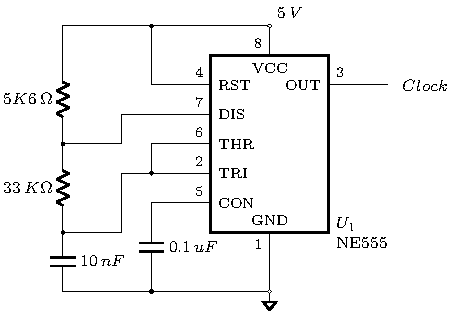
\includegraphics[scale=0.8]{Ejercicio8/Circuitos/Clock.pdf}
\caption{Generador de clock}
\label{fig:Clock}
\end{figure}

Por otro lado, para mostrar la posición al usuario se utilizaron dos displays previo paso por un decodificador BCD a display 7 segmentos($CD4511$).



\subsection{Métodos de control}

\subsubsection{Enable contador de posición}
La entrada de habilitación de los contadores de posición va a estar dado por la salida de una compuerta AND($74HC08$) cuyas entradas son la salida del comparador entre la rampa y el joystick y la señal que indica que ambos números son iguales como se puede ver en la figura (\ref{fig:enable}). Esta última será un pulso que estará alto durante todo un ciclo de clock mientras que la duración del pulso del comparador estará dado por la tensión del joystick, teniendo una duración de entre aproximadamente un pulso para el caso en el que caigan $5\,V$ en el joystick y un pulso muy breve cuando la tensión que caiga en dicho componente sea cercana a $0\,V$. 

\par
\begin{figure}[H]
\centering
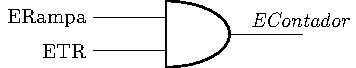
\includegraphics[scale=0.8]{Ejercicio8/Circuitos/Enable.pdf}
\caption{Enable del contador de posición}
\label{fig:enable}
\end{figure}

Por otro lado, el decoder presenta una entrada LatchEnable/Strobe que permite guardar un valor(activo alto) o para tomar el valor presente en sus entradas(activo bajo) respectivamente. Dicho comportamiento es complementario del enable presentado más arriba, es decir, se deberá guardar el número, que es presentado en el display, cuando la salida esté en bajo. Por ende se implementa la siguiente conexión que nos definirá en que momento se refrescan los display.
\par
\begin{figure}[H]
\centering
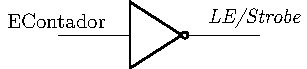
\includegraphics[scale=0.8]{Ejercicio8/Circuitos/not.pdf}
\caption{LatchEnable del decoder}
\label{fig:not}
\end{figure}

\subsubsection{Reset contador de posición}
El sistema de conteo debe reiniciarse cada vez que sea necesario volver a contar, dicho momento dependerá de la tasa de refresco a la que se esté trabajando. Dicho instante estará determinado por dos condiciones, la primera que la rampa esté a un nivel de tensión de $0\,V$ y la otra que el enable del contador de posición  esté alto. Para determinar la primer condición, se utilizará un comparador($LM339$) entre la tensión de la rampa y tierra como se puede ver en la figura (\ref{fig:Reset}).

\begin{figure}[H]
\centering
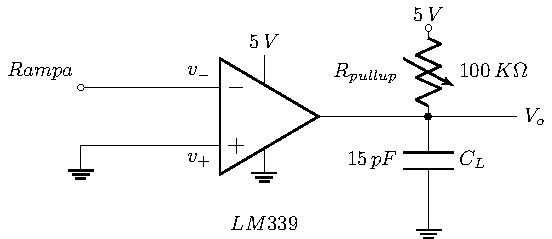
\includegraphics[scale=0.8]{Ejercicio8/Circuitos/Reset.pdf}
\caption{Reset}
\label{fig:Reset}
\end{figure}


\subsection{Conclusiones}
Como primera conclusión, visto en retrospectiva fue un error haber implementado todo el circuito en la mismo PCB, debido a que al aumentar la superficie del circuito la aparición de errores, más que nada de impresión, fue notoria. También, se vuelve mucho más difícil encontrar dichos errores y corregirlos debido a una alta densidad de componentes y pistas. Una modularización en distintas placas, como mínimo una para la parte digital y otra para la analógica, huiese permitido una mayor eficiencia y claridad al momento de implementar la placa. \par Sin embargo, consideramos que esto se debe a los métodos de fabricación de baja tecnología e imprecisos al alcance de los integrantes de este grupo, una falta de experiencia previa en un proyecto tan complejo y errores en el diseño, lo cual no implica que dicho enfoque sea un error per se. \par 
Respecto a la injerencia del ruido en el circuito, la misma fue baja por lo que se considera que las medidas tomadas para paliar dicho incoveniente cumplieron con su finalidad. \par 
Respecto del circuito implementado para determinar la tasa de refresco, se cree que se podría haber implementado y/o optimizado de otra forma ya que termina siendo poco amigable y claro para el usuario debido al ingreso manual de un valor que no termina siendo la tasa de refresco deseada. Se considero diseñar un circuito lógico para hacer dicha conversión de lo ingresado por el usuario a su tasa de refresco equivalente pero se descartó ya que requería, no pudiendo usar lógica programable, un circuito complejo de compuertas discretas que sumaba en complejidad pero no en profundidad o en manejo de conceptos al trabajo.\par 
 Visto en retrospectiva, lo ideal hubiese sido implementar el ingreso de la tasa de refresco mediante la forma analógica, el potenciómetro, con un display asociado que mostrará la tasa de refresco asociada a esa posición del resistor variable. Siendo esta la opción más amigable al usuario y pudiendo reutilizar otros elementos dentro de nuestro diseño, como la rampa. \par 
 
